\documentclass{article}
\usepackage[T2A]{fontenc}
\usepackage[utf8]{inputenc}
\usepackage[russian]{babel}
\usepackage{amsmath}
\usepackage{amssymb}
\usepackage[makeroom]{cancel}
\usepackage{hyphenat}
\hyphenation{ма-те-ма-ти-ка вос-ста-нав-ли-вать}
\usepackage{graphicx}

\title{Домашнее Задание №1}
\author{Дарвин Эдлеазар Пиче Круз}

\begin{document}

\maketitle

\section*{1.1}

Для каждой из рассматриваемых дальше функций f(n) найдите
наиболее компактно записываемую g(n), что $f(n) = \Theta(g(n))$ и докажите это соотношение.

%1.1

%a

\bigskip
\bigskip
\textbf{a)} $f(n) = 7n^2 - 7(n - 3)^2$

\textbf{Решение}
\begin{equation*}
    f(n) = 7n^2 - 7n^2 +42n - 63 \longrightarrow f(n) = 42n - 63
\end{equation*}

\textbf{Ответ:} $f(n) = \Theta(n)$

\textbf{Доказательство:}

Возьмём $c_2 = 42$ и $c_1 = 1$ тогда: $c_1 \cdot n \leq f(n) \leq c_2 \cdot n \; \forall n > n_0$ 

%b
\bigskip
\bigskip
\textbf{b) $f(n) = 5n + 2\sqrt[3]{n}$}

\textbf{Решение}
\begin{equation*}
    f(n) = 5n + 2n^{\frac{1}{3}}
\end{equation*}

\textbf{Ответ:} $f(n) = \Theta(n)$

\textbf{Доказательство:}

Возьмём $c_2 = 7$ и $c_1 = 1$ тогда: $c_1 \cdot n \leq f(n) \leq c_2 \cdot n \; \forall n > n_0$ 

%c
\bigskip
\bigskip
\textbf{c) $f(n) = 10(n + 1)^2 + 3(n - 2)$}

\textbf{Решение}
\begin{equation*}
    f(n) = 10n^2 + 20n + 10 + 3n - 6 \longrightarrow f(n)=10n^2+23n + 4
\end{equation*}

\textbf{Ответ:} $f(n) = \Theta(n^2)$

\textbf{Доказательство:}

Возьмём $c_2 = 37$ и $c_1 = 1$ тогда: $c_1 \cdot n^2 \leq f(n) \leq c_2 \cdot n^2 \; \forall n > n_0$ 

%d
\bigskip
\bigskip
\textbf{d) $f(n) = log(\sqrt{n}) + \sqrt{log(n)}$}

\textbf{Решение}
\begin{equation*}
    f(n) = log\left(n^{\frac{1}{2}}\right) + (log(n))^{\frac{1}{2}} \longrightarrow f(n) = \dfrac{1}{2} log(n) + (log(n))^{\frac{1}{2}}
\end{equation*}

\textbf{Ответ:} $f(n) = \Theta(log(n))$

\textbf{Доказательство:}

Возьмём $c_2 = 4$ и $c_1 = \dfrac{1}{2}$ тогда: $c_1 \cdot log(n) \leq f(n) \leq c_2 \cdot log(n) \; \forall n > n_0$ 

%e
\bigskip
\bigskip
\textbf{e) $f(n) = n\cdot 3^{n + 1} + n^{10}$}

\textbf{Ответ:} $f(n) = \Theta(n\cdot 3^{n + 1})$

\textbf{Доказательство:}

Возьмём $c_2 = 7000$ и $c_1 = 1$ тогда: $c_1 \cdot n\cdot 3^{n + 1} \leq f(n) \leq c_2 \cdot n\cdot 3^{n + 1} \; \forall n > n_0$


%f
\bigskip
\bigskip
\textbf{f) $f(n) = \dfrac{10n^2 + 2}{7n - 1}$}

\textbf{Решение}
\begin{equation*}
    10n^2 + 2 = (7n - 1)\left(10n + \dfrac{10}{49}\right) + \dfrac{108}{49}
\end{equation*}
\begin{equation*}
    \dfrac{10n^2 + 2}{7n - 1} = 10n + \dfrac{10}{49} + \dfrac{108}{49(7n - 1)}
\end{equation*}

\textbf{Ответ:} $f(n) = \Theta(n)$

\textbf{Доказательство:}

Возьмём $c_2 = 100$ и $c_1 = 1$ тогда: $c_1 \cdot n \leq f(n) \leq c_2 \cdot n \; \forall n > n_0$ 


%g
\bigskip
\bigskip
\textbf{g) $f(n) = log(2n log(n))$}

\textbf{Решение}
\begin{equation*}
    f(n) = log(2) + log(n) + log(log(n))
\end{equation*}

\textbf{Ответ:} $f(n) = \Theta(log(n))$

\textbf{Доказательство:}

Возьмём $c_2 = 100$ и $c_1 = 1$ тогда: $c_1 \cdot log(n) \leq f(n) \leq c_2 \cdot log(n) \; \forall n > n_0$ 


%1.2

\section*{1.2}
Для следующих пар функций f(n) и g(n) покажите, верно ли, что
$f(n) = O(g(n))$ и докажите свой ответ.


%a
\bigskip
\bigskip
\textbf{a)}
\begin{equation*}
    f(n) = log(n)
\end{equation*}
\begin{equation*}
    g(n) = \sqrt{n}
\end{equation*}

\textbf{Ответ:} Верно

\textbf{Доказательство:}

$\forall c>0 \; f(n) \leq c \cdot g(n) \; \; \forall n > n_0$


%b
\bigskip
\bigskip
\textbf{b)}
\begin{equation*}
    f(n) = n\sqrt{n} log(n)
\end{equation*}
\begin{equation*}
    g(n) = n \log^3n
\end{equation*}

\textbf{Ответ:} Неверно

\textbf{Доказательство:}

$\nexists c :  \; f(n) \leq c \cdot g(n) \; \; \forall n > n_0$ т. е. Неважно, насколько большим становится c, всегда существует n, так что $f(n) > c \cdot g(n)$


%c
\bigskip
\bigskip
\textbf{c)}
\begin{equation*}
    f(n) = n)
\end{equation*}
\begin{equation*}
    g(n) = (\log{n})^{\log{n}}
\end{equation*}

\textbf{Ответ:} Неверно

\textbf{Доказательство:}

$\nexists c :  \; f(n) \leq c \cdot g(n) \; \; \forall n > n_0$ т. е. Неважно, насколько большим становится c, всегда существует n, так что $f(n) > c \cdot g(n)$ например: если $c = 10000$, возьмём $n = 100000$ и тогда $f(n) > c \cdot g(n)$


%1.3

\section*{1.3}
Время работы некоторого алгоритма задано следующим рекуррентным соотношением. Найдите $\Theta$-асимптотику времени работы
этого алгоритма, построив дерево рекурсивных вызовов.

%a
\bigskip
\bigskip
\textbf{a)}
\begin{equation*}
    T(n) = T(n - 1) + 2n^2
\end{equation*}

%insertar foto 1
\begin{figure}[h]
    \centering
    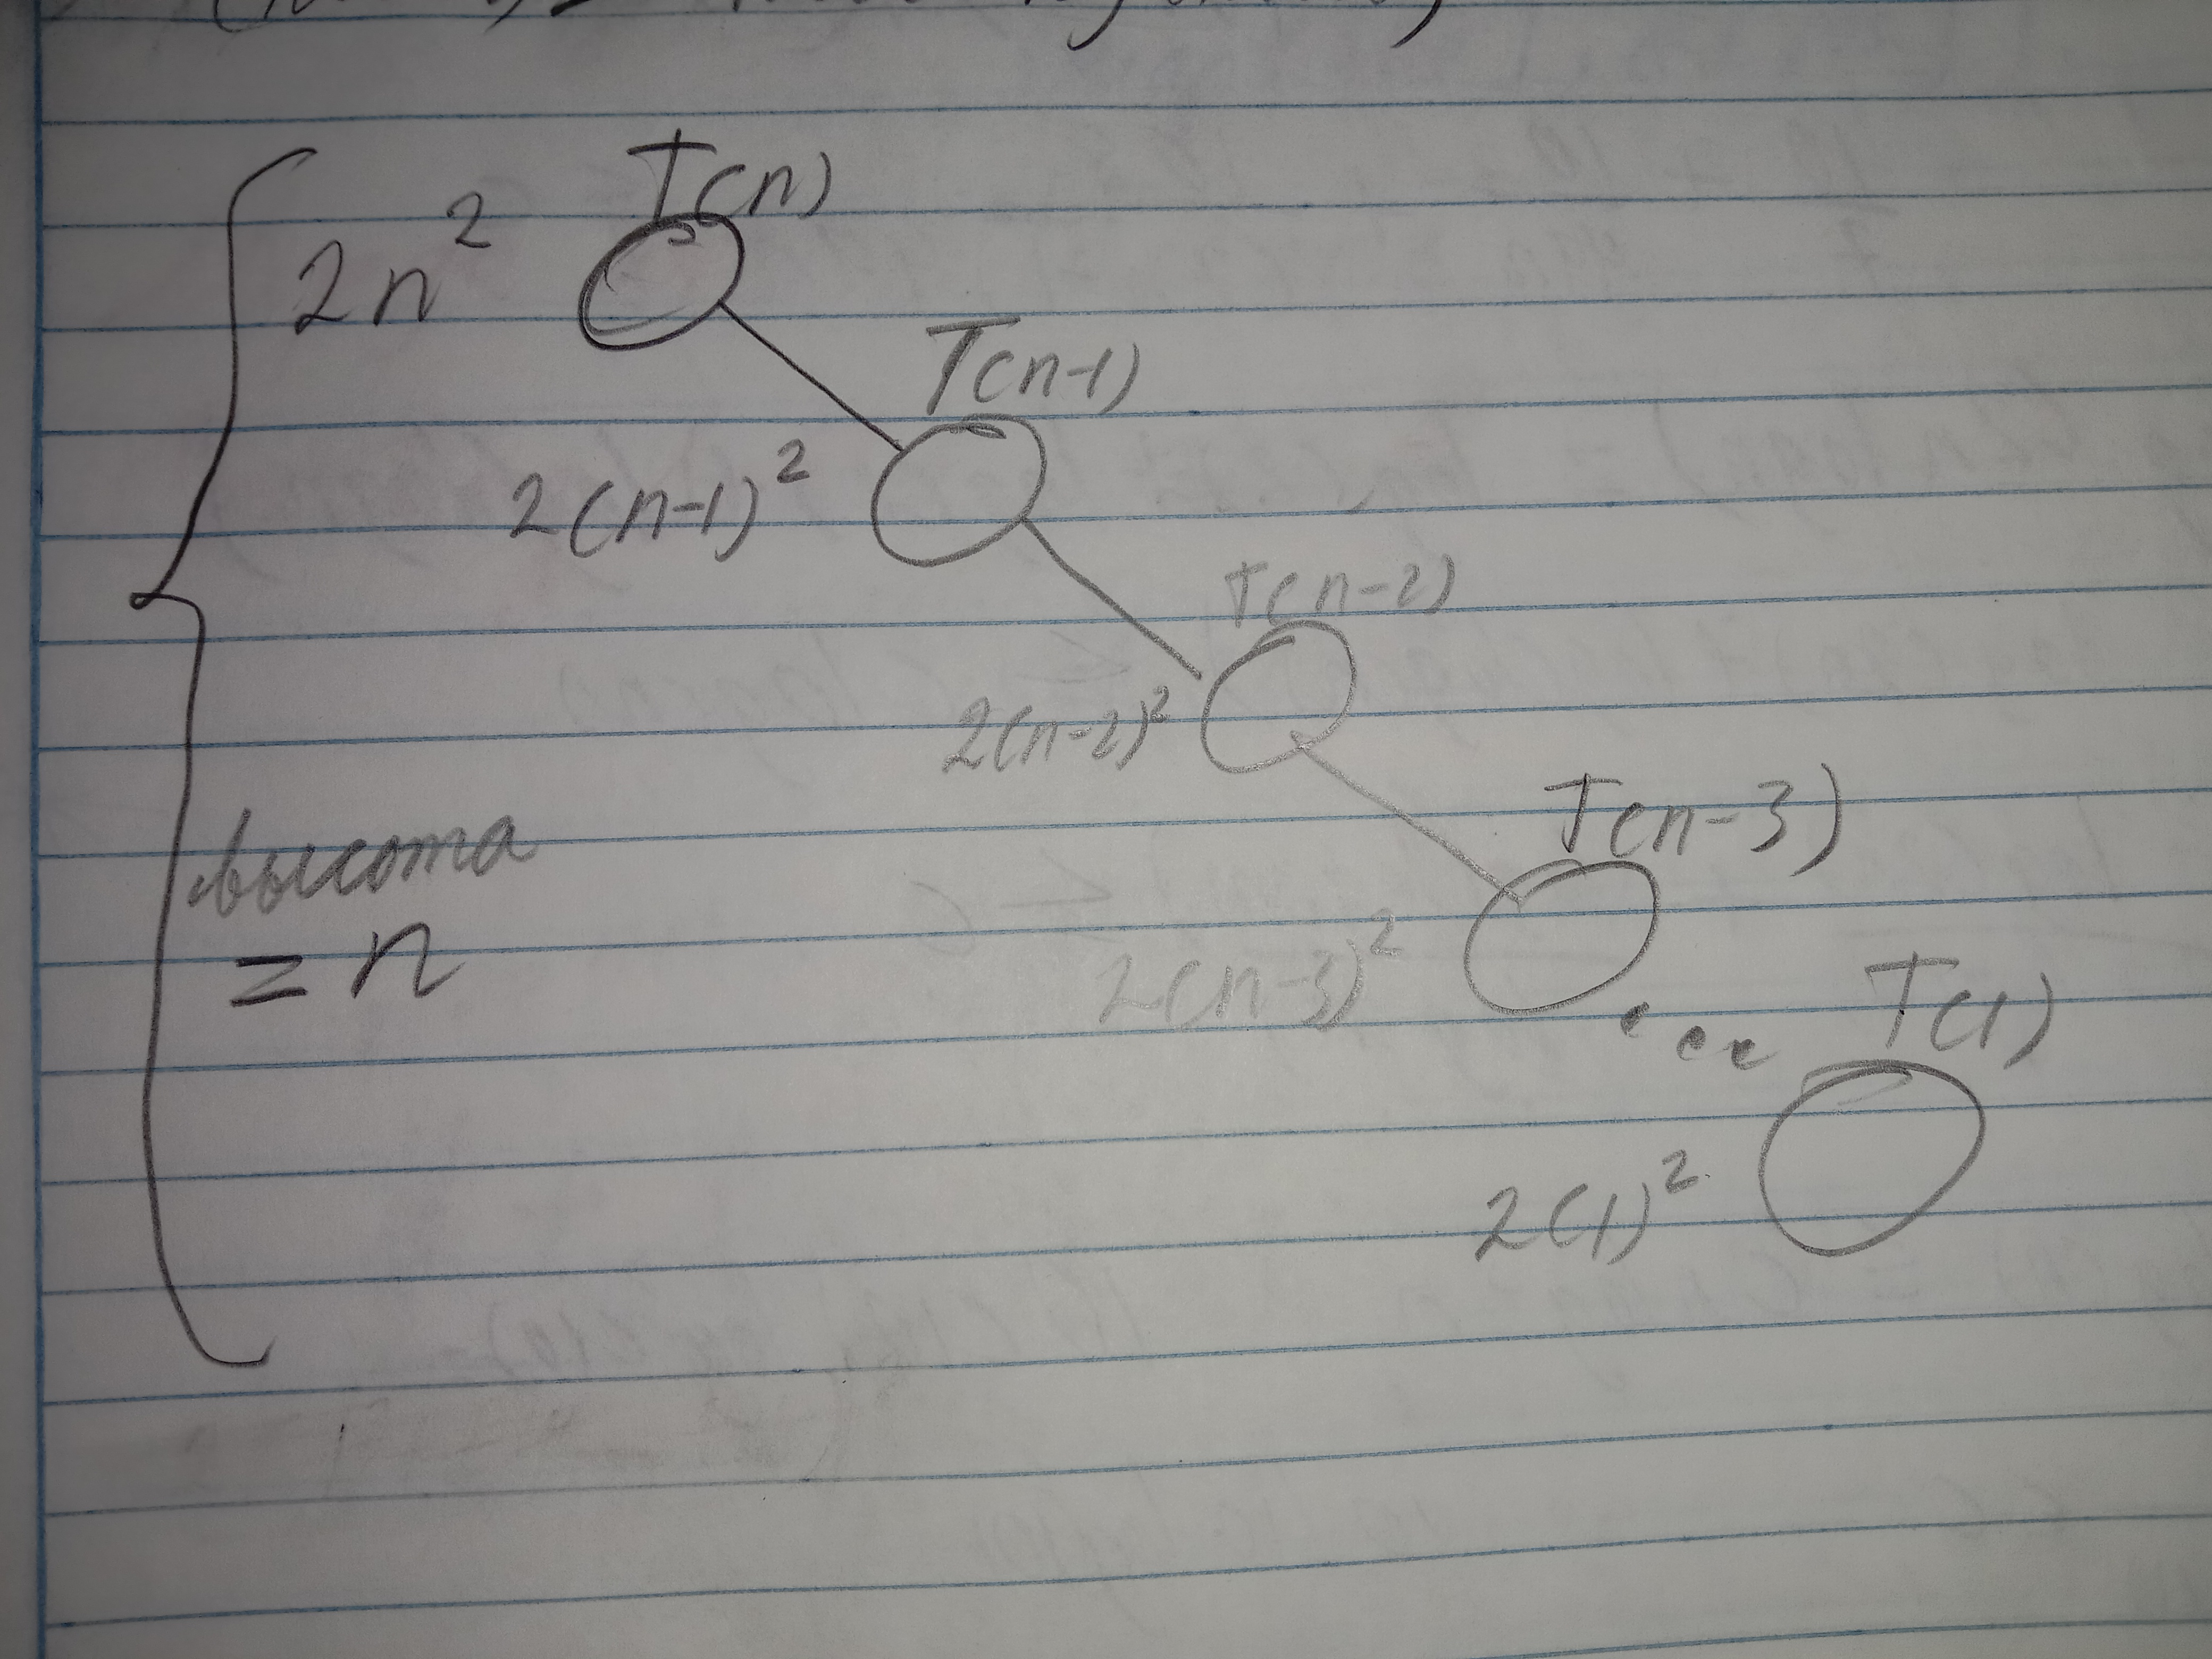
\includegraphics[width=10cm, height=10cm]{1.jpg}
    \caption{}
    \label{fig:my_label}
\end{figure}

\newpage

так как высота дерева = n (рис 1):

\begin{equation*}
    T(n) = 2*(1^2+2^2+3^2+...+n^2) = \dfrac{n(n+1)(2n+1)}{6} = \Theta(n^3) 
\end{equation*}

%b
\bigskip
\bigskip
\textbf{b)}
\begin{equation*}
    T(n) = T(\frac{n}{2}) + n
\end{equation*}

%insertar foto
\begin{figure}[h]
    \centering
    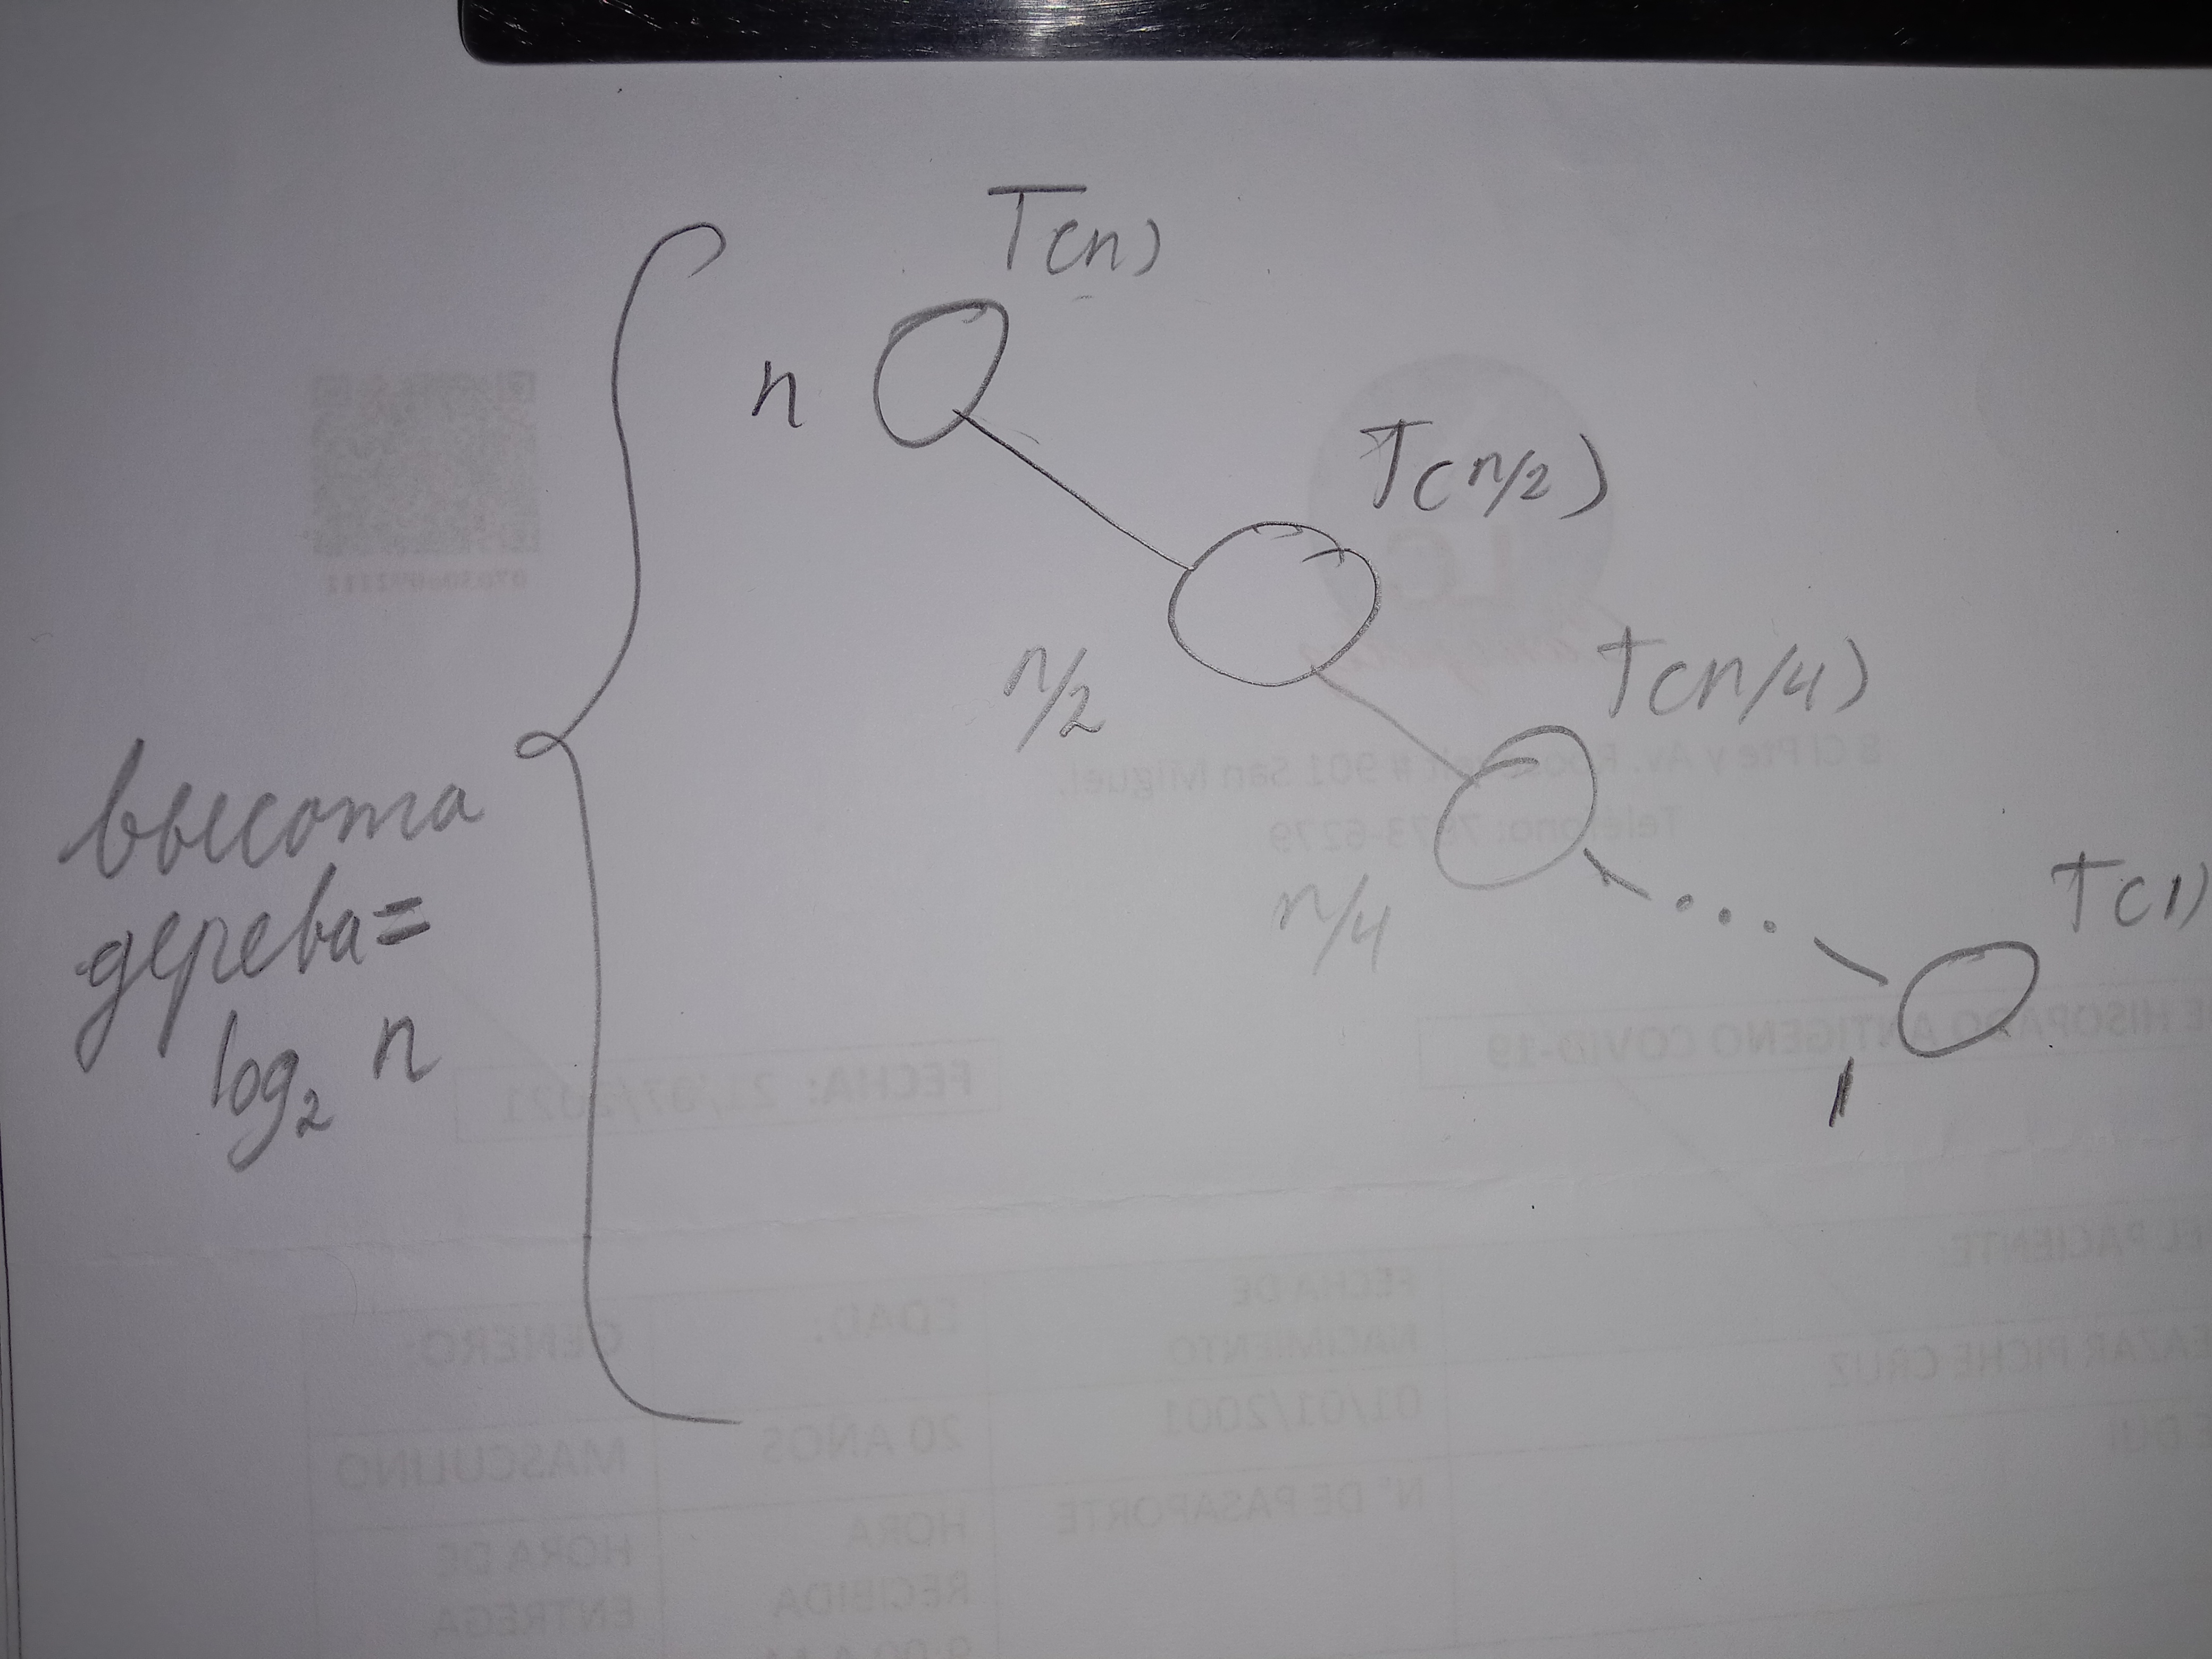
\includegraphics[width=10cm, height=10cm]{2.jpg}
    \caption{}
    \label{fig:my_label}
\end{figure}

\newpage

так как высота дерева $= log(n)$ (рис 2):

\begin{equation*}
    T(n) = n+\dfrac{n}{2}+\dfrac{n}{4}+...\dfrac{n}{2^{log(n)}}= \cancel{n}\cdot \dfrac{2^{log(n)} + 2^{log(n) - 1} + \dots + 2^0}{\cancel{2^{log(n)}}}
\end{equation*}
\begin{equation*}
    = 2^{log(n) + 1} - 1 = 2^{log(n)} * 2 - 1 = 2n - 1 = \Theta(n) 
\end{equation*}

%c
\bigskip
\bigskip
\textbf{c)}
\begin{equation*}
    T(n) = 3T\left(\frac{n}{2}\right) + 2
\end{equation*}

%insertar foto
\begin{figure}[h]
    \centering
    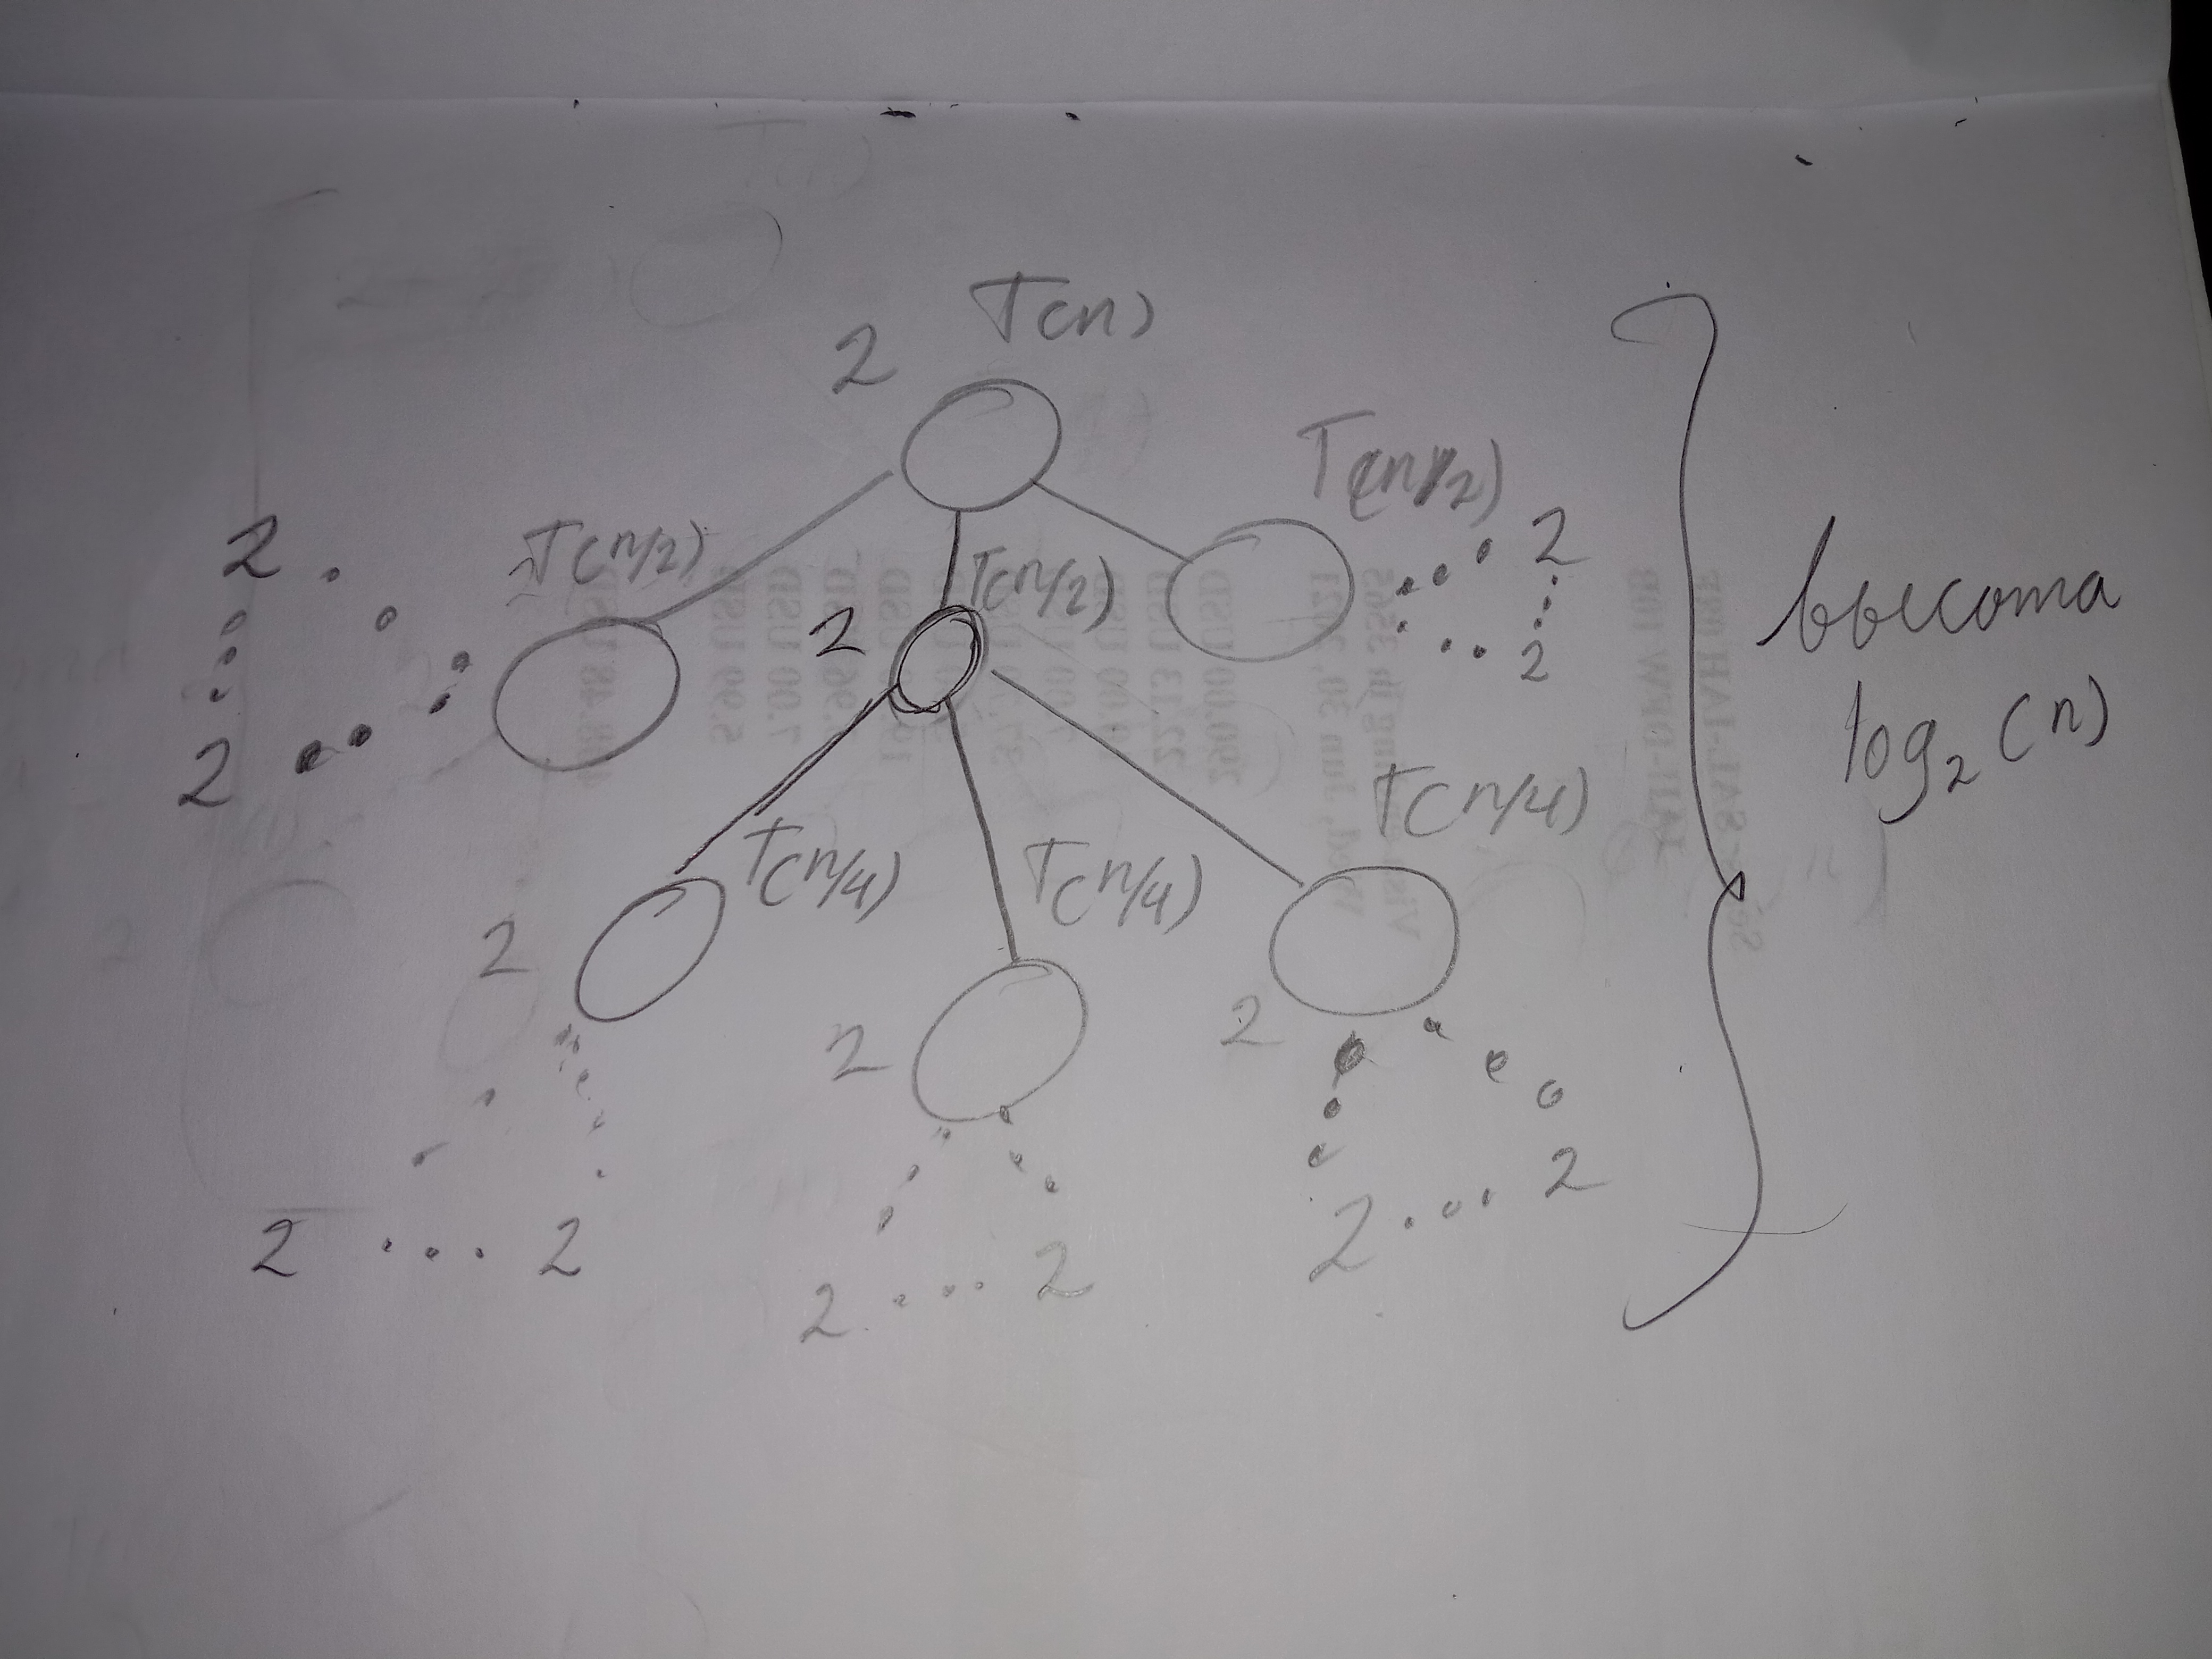
\includegraphics[width=10cm, height=10cm]{3.jpg}
    \caption{}
    \label{fig:my_label}
\end{figure}

\newpage

мы подсчитываем количество узлов дерева, и это количество раз, когда мы суммируем 2.\newline
так как высота дерева $= log(n)$ (рис 3):

\begin{equation*}
    T(n) = 2*3^{log(n)} = 2*3^{\dfrac{\log_{3}{n}}{\log_{3}{2}}} = \sqrt[\log_{3}{2}]{3^{\log_{3}{n}}} = \sqrt[\log_{3}{2}]{n}
\end{equation*}
так как $\log_{3}{2} \approx 1$
\begin{equation*}
    T(n)=\Theta(n)
\end{equation*}


%d
\bigskip
\bigskip
\textbf{d)}
\begin{equation*}
    T(n) = T\left(\frac{n}{3}\right) + \log n
\end{equation*}

%insertar foto

\begin{figure}[h]
    \centering
    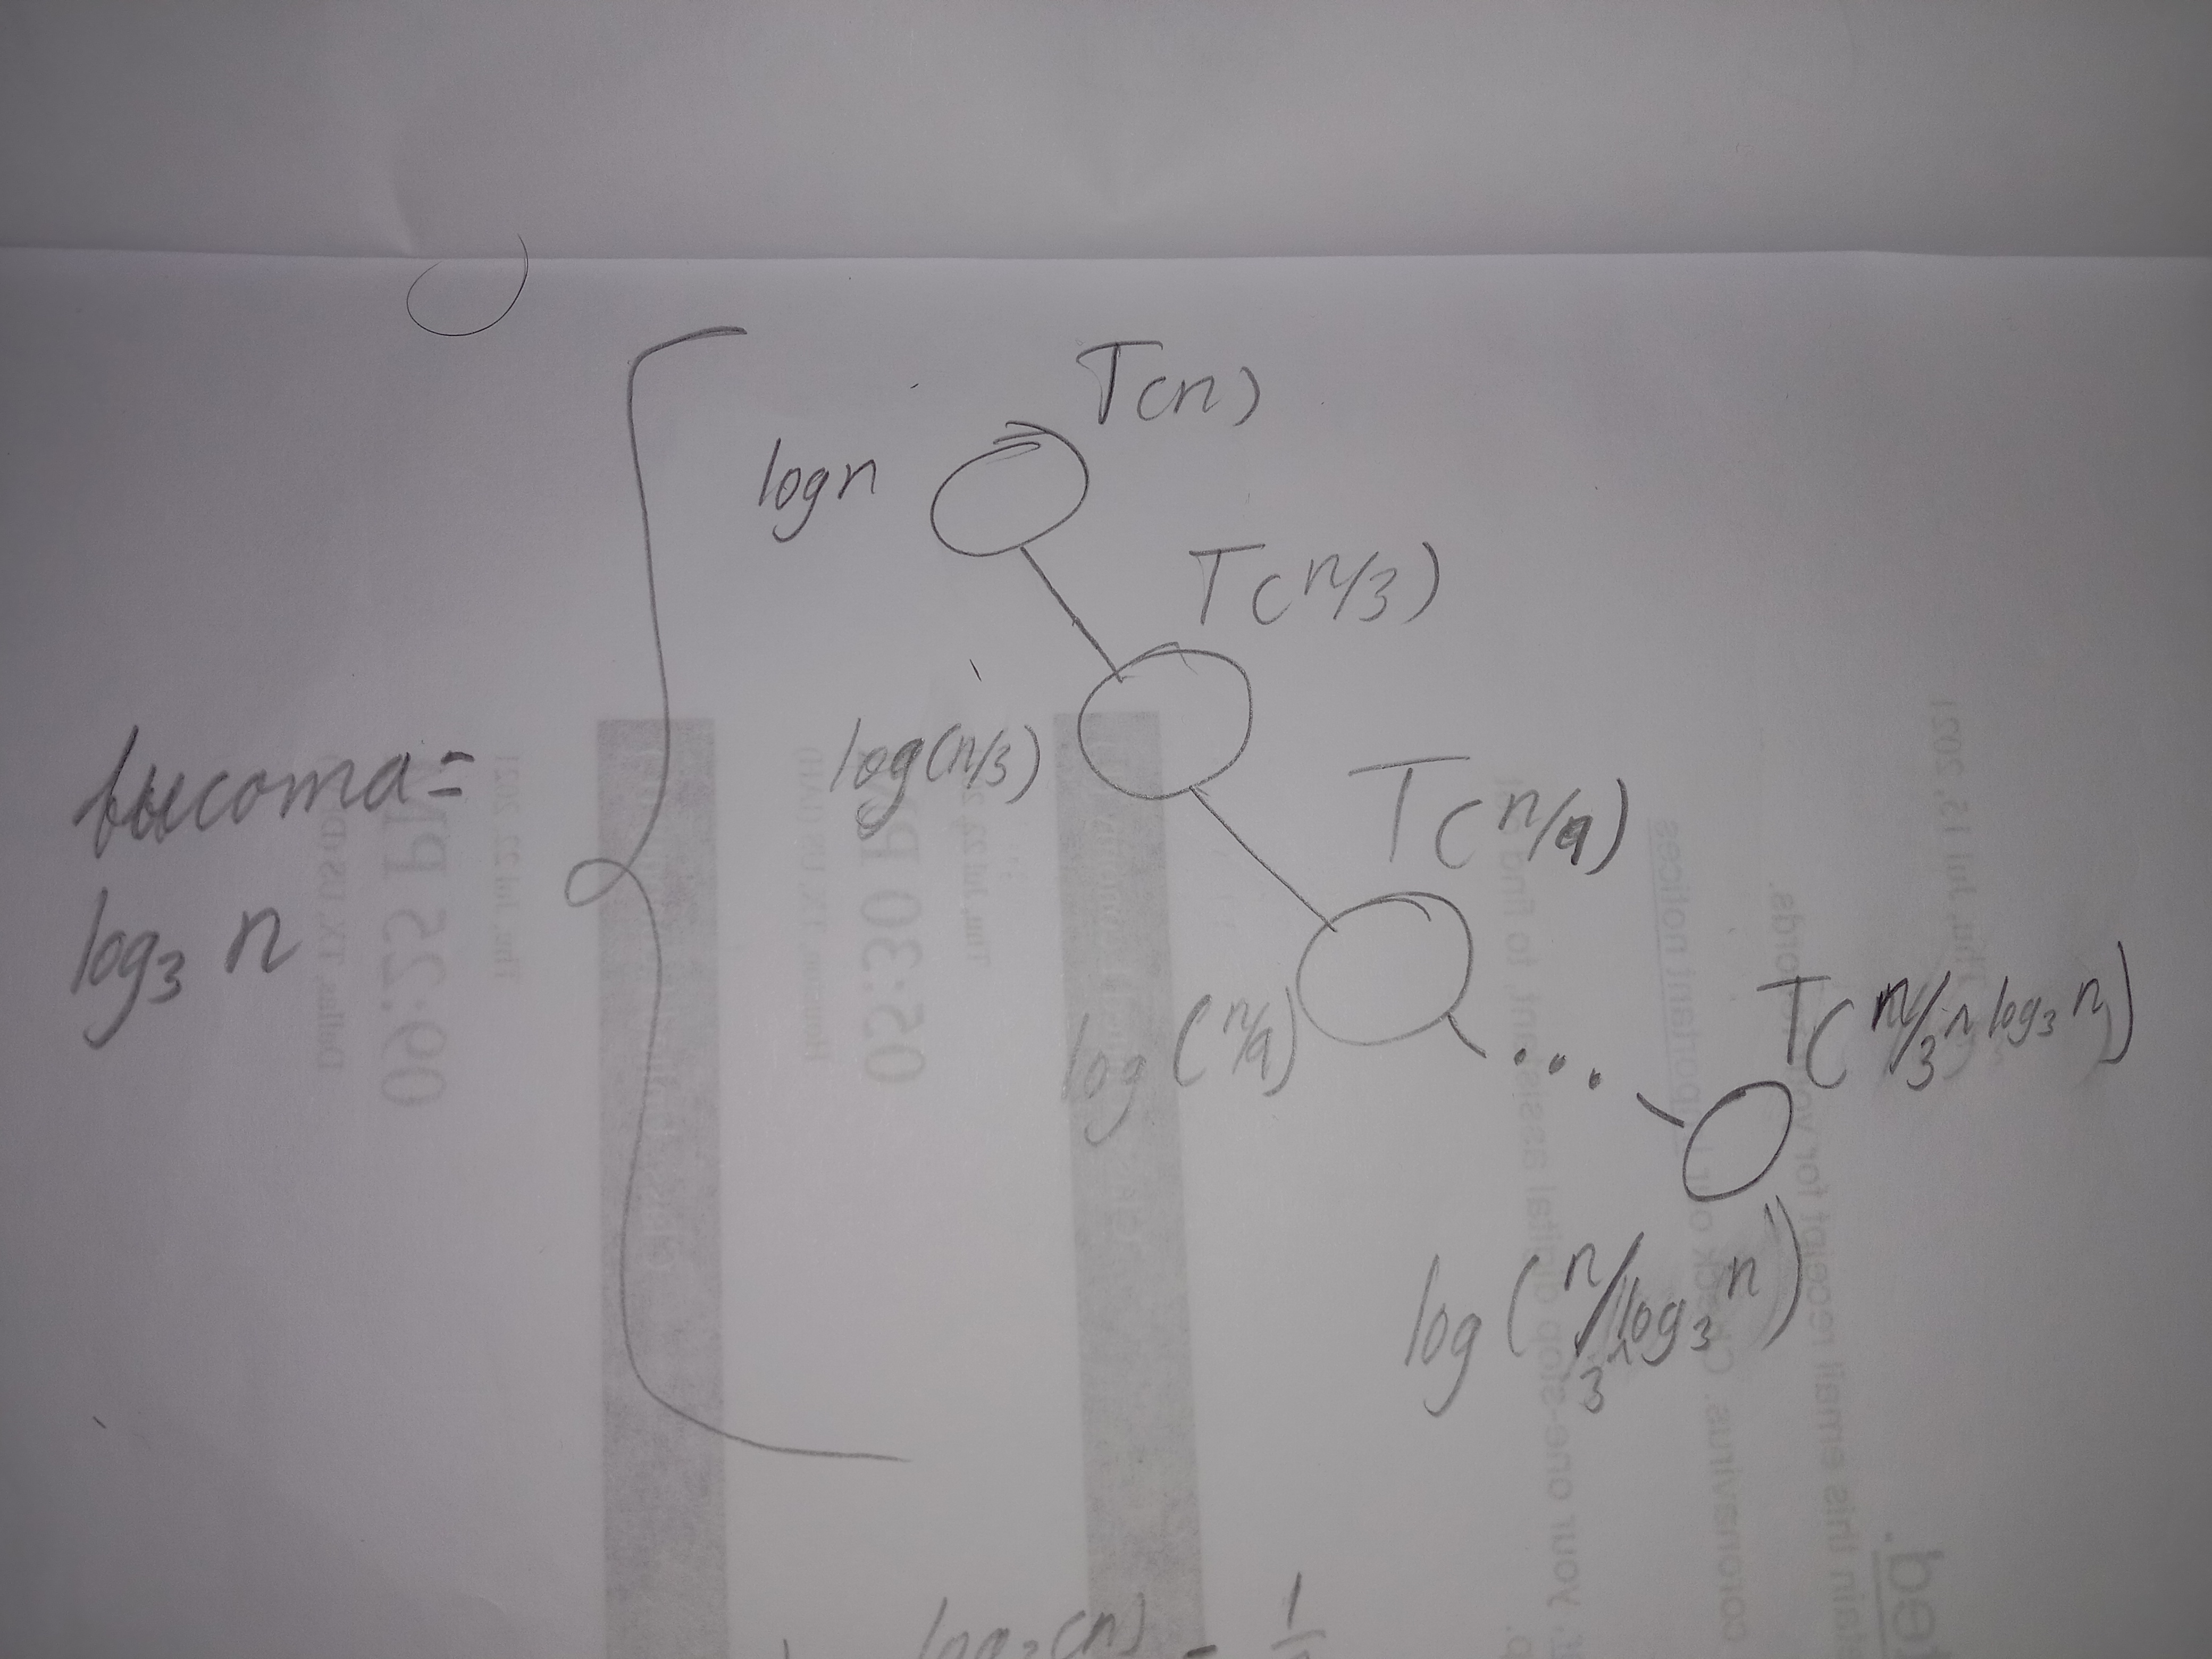
\includegraphics[width=10cm, height=10cm]{4.jpg}
    \caption{}
    \label{fig:4}
\end{figure}

\newpage

так как высота дерева $= \log_{3}(n)$ (рис 4):

\begin{equation*}
    T(n) = \log n + \log \left(\dfrac{n}{3}\right) + \log \left(\dfrac{n}{9}\right) + \cdots + \log \left(\dfrac{n}{3^{\log_{3}(n)}} \right)
\end{equation*}
\begin{equation*}
    T(n) = \log \left(\dfrac{n^{\log_{3}(n)}}{3^{1+2+3+\cdots+\log_{3}(n)}}\right)
\end{equation*}
\begin{equation*}
    T(n) = \log \left(\dfrac{n^{\log_{3}(n)}}{\sqrt{n^{\log_{3}(n) + 1}}}\right)
\end{equation*}
\begin{equation*}
    T(n) = \log_{3}(n) \log \left(n\right) - \left(\dfrac{\log_{3}(n) + 1}{2} \right) \log \left(\sqrt{n}\right)
\end{equation*}
\begin{equation*}
    T(n)=\Theta(\log_{3}(n) \log (n))
\end{equation*}


%1.4

\section*{1.4}
Докажите следующие утверждения по индукции. В качестве базы
во всех пунктах можно считать, что $T(1) = 1.$

%a
\bigskip
\bigskip
\textbf{a)}
\begin{equation*}
    T(n) = 2T(\sqrt{n}) + 1 \longrightarrow T(n) = \mathcal{O} (\log (n))
\end{equation*}

\textbf{Решение}

Попровуем с $T(2) = 2T(\sqrt{2})+1 \leq c\log (2) \longrightarrow 2(1) + 1 \leq c$.
Возьмём $c = 3$ и уравнение удовлетворяется.

\begin{equation*}
    \forall n > 1 : \; \; 2T(\sqrt{n}) + 1 \leq c\log n
\end{equation*}
Для $n + 1$:
\begin{equation*}
    T(n + 1) = 2T(\sqrt{n + 1}) + 1 =  2(2T(\sqrt{n}) + 1) + 1 = 4T(\sqrt{n}) + 3
\end{equation*}
Так как $T(\sqrt{n}) + 3 \leq c\log (n)$ при $c$ достаточно большой:
$T(n) = 2T(\sqrt{n}) + 1 \;\; T(n) = \mathcal{O} (\log (n))$


%b
\bigskip
\bigskip
\textbf{b)}
\begin{equation*}
    T(n) = 2T\left(\frac{n}{2}\right) + n \longrightarrow T(n) = \mathcal{O} (n\log (n))
\end{equation*}

\textbf{Решение}

Попровуем с $T(2) = 2T(1) + 2 \leq c*2\log (2) \longrightarrow 4 \leq 2*c$.
Возьмём $c = 2$ и уравнение удовлетворяется.

\begin{equation*}
    \forall n > 1 : \; \; 2T\left(\frac{n}{2}\right) + n \leq cn\log n
\end{equation*}
Для $n + 1$:
\begin{equation*}
    T(n + 1) = 2T\left(\frac{n + 1}{2}\right) + n + 1 =  2(2T\left(\frac{n}{2}\right) + n) + n + 1 = 4T\left(\frac{n}{2}\right) + 3n + 1
\end{equation*}
Так как $4T\left(\frac{n}{2}\right) + 3n + 1 \leq cn\log (n)$ при $c$ достаточно большой:
$T(n) = 2T\left(\frac{n}{2}\right) + n \longrightarrow T(n) = \mathcal{O} (n\log (n))$

%c
\bigskip
\bigskip
\textbf{c)}
\begin{equation*}
    T(n) = 2T\left(\frac{n}{2}\right) + n \longrightarrow T(n) = \Omega (n\log (n))
\end{equation*}

\textbf{Решение}

Попровуем с $T(2) = 2T(1) + 2 \geq c*2\log (2) \longrightarrow 4 \geq 2*c$.
Возьмём $c = 1$ и уравнение удовлетворяется.

\begin{equation*}
    \forall n > 1 : \; \; 2T\left(\frac{n}{2}\right) + n \geq cn\log n
\end{equation*}
Для $n + 1$:
\begin{equation*}
    T(n + 1) = 2T\left(\frac{n + 1}{2}\right) + n + 1 =  2(2T\left(\frac{n}{2}\right) + n) + n + 1 = 4T\left(\frac{n}{2}\right) + 3n + 1
\end{equation*}
Так как $T\left(\frac{n}{2}\right) + 3n + 1 \geq cn\log (n)$при $c$ достаточно маленький:
$T(n) = 2T\left(\frac{n}{2}\right) + n \longrightarrow T(n) = \Omega (n\log (n))$

%d
\bigskip
\bigskip
\textbf{d)}
\begin{equation*}
    T(n) = 3T\left(\frac{n}{2}\right) + 1 \longrightarrow T(n) = \Omega (n)
\end{equation*}

\textbf{Решение}

Попровуем с $T(2) = 3T(1) + 1 \geq 2c \longrightarrow 4 \geq 2*c$.
Возьмём $c = 1$ и уравнение удовлетворяется.

\begin{equation*}
    \forall n > 1 : \; \; 3T\left(\frac{n}{2}\right) + 1 \geq cn
\end{equation*}
Для $n + 1$:
\begin{equation*}
    T(n + 1) = 3T\left(\frac{n + 1}{2}\right) + 1 =  3\left(3T\left(\frac{n}{2}\right) + 1\right) + 1 = 9T\left(\frac{n}{2}\right) + 4
\end{equation*}
Так как $9T\left(\frac{n}{2}\right) + 4 \geq cn$  при $c$ достаточно маленький:\\
$T(n) = 3T\left(\frac{n}{2}\right) + 1 \longrightarrow T(n) = \Omega (n)$



%1.5

\section*{1.5}
Докажите, что 
\begin{equation*}
    \sum_{t=1}^{n}\dfrac{1}{t}=\Omega (\log n)
\end{equation*}

\textbf{Решение}

Используя метод интегралами, так как площадь под кривой $\leq$ нашей суммы

\begin{equation*}
    \sum_{t=1}^{n}\dfrac{1}{t} \geq \int_{1}^{n} \dfrac{1}{n} dn
\end{equation*}
\begin{equation*}
    \sum_{t=1}^{n}\dfrac{1}{t} \geq \log (n) - \cancel{\log (1)} + C
\end{equation*}
\begin{equation*}
    \sum_{t=1}^{n}\dfrac{1}{t} \geq C_2\log (n)
\end{equation*}
При $C_2$ Достаточно маленький, уравнение удовлетворяется




%1.6

\section*{1.6}
 6. Докажите или опровергните следующие утверждения. В качестве
опровержения достаточно привести контрпример и показать, почему для него утверждение не выполняет


%a
\bigskip
\bigskip
\textbf{a)}
\begin{equation*}
    f(n) = \mathcal{O}(g(n)) \longrightarrow f^2(n) = \mathcal{O}(g(n))
\end{equation*}

\textbf{Решение}
так как
\begin{equation*}
    f(n) \leq c(g(n))
\end{equation*}
\begin{equation*}
    f(n) \cdot f(n) \leq c(g(n)) \cdot f(n) \leq c(g(n)) \cdot c(g(n))
\end{equation*}
\begin{equation*}
    f^2(n) \leq c^2(g^2(n))
\end{equation*}
Возьмём $c_2 = c^2$
\begin{equation*}
    f^2(n) \leq c_2(g^2(n))
\end{equation*}
\textbf{Ответ:} Верно



%b
\bigskip
\bigskip
\textbf{b)}
\begin{equation*}
    f(n) = \mathcal{O}(g(n)) \longrightarrow 2^{f(n)} = \mathcal{O}(2^{g(n)})
\end{equation*}

\textbf{Решение}
так как
\begin{equation*}
    f(n) \leq cg(n)
\end{equation*}
\begin{equation*}
    2^{f(n)} \leq 2^{cg(n)}
\end{equation*}
\begin{equation*}
    2^{f(n)} \leq 2^c*2^{g(n)}
\end{equation*}
Возьмём $c_2 = 2^c$
\begin{equation*}
    2^{f(n)} \leq c_2 \cdot 2^{g(n)}
\end{equation*}
\textbf{Ответ:} Верно


%c
\bigskip
\bigskip
\textbf{c)}
\begin{equation*}
    f(n) = \mathcal{O}(g(n)) \longrightarrow \log (f(n)) = \mathcal{O}(\log (g(n)))
\end{equation*}

\textbf{Решение}
так как
\begin{equation*}
    f(n) \leq cg(n)
\end{equation*}
\begin{equation*}
    \log (f(n)) \leq \log (cg(n))
\end{equation*}
\begin{equation*}
    \log (f(n)) \leq \log c + \log (g(n))
\end{equation*}
Возьмём $c_2$ Достаточно болшой, такой что:
\begin{equation*}
    \log (f(n)) \leq c_2\log (g(n))
\end{equation*}
\textbf{Ответ:} Верно
\end{document}
